\documentclass[dvisvgm,border=2pt]{standalone}
% Shared by every figure. Two colours only: black becomes the text colour of
% whatever theme the app is in, and `accent` becomes the brand — see
% scripts/build-figures.mjs. Everything else is done with opacity.
\usepackage{amsmath}
\usepackage{amssymb}
\usepackage{tikz}
\usepackage{pgfplots}
\pgfplotsset{compat=1.18}
\usetikzlibrary{arrows.meta,positioning,calc,backgrounds,fit,patterns.meta}
\definecolor{accent}{RGB}{255,0,255}
\pgfplotsset{
  every axis/.append style={
    axis lines=left,
    axis line style={draw opacity=0.35},
    tick style={draw opacity=0.35},
    tick label style={font=\scriptsize,opacity=0.7},
    label style={font=\scriptsize,opacity=0.7},
    legend style={draw=none,fill=none,font=\scriptsize},
    every axis plot/.append style={line width=0.7pt},
  },
}
\tikzset{
  every picture/.style={font=\scriptsize},
  faint/.style={opacity=0.3},
  quiet/.style={opacity=0.55},
  box/.style={draw,opacity=0.35,rounded corners=2pt,inner sep=4pt},
  hot/.style={accent},
}

\begin{document}
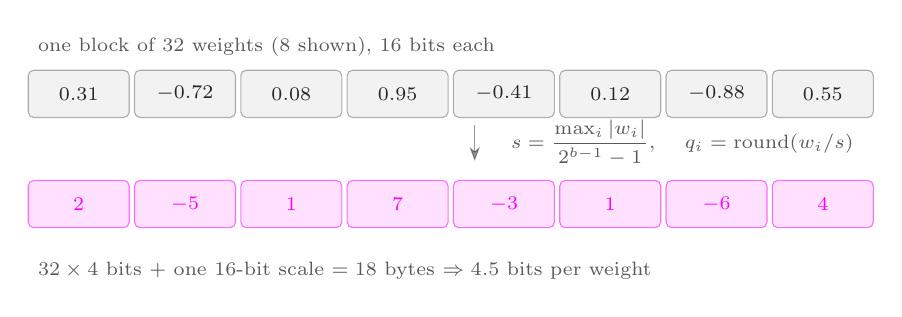
\begin{tikzpicture}[x=1.35cm,y=1cm]
  \node[anchor=west,opacity=0.65] at (0,2.5) {one block of 32 weights (8 shown), $16$ bits each};
  \foreach \w [count=\i from 0] in {0.31,-0.72,0.08,0.95,-0.41,0.12,-0.88,0.55}{
    \draw[opacity=0.3,rounded corners=2pt,fill,fill opacity=0.05]
      (\i,1.6) rectangle ++(0.95,0.6);
    \node[opacity=0.85] at (\i+0.475,1.9) {$\w$};
  }
  \draw[opacity=0.4,-{Stealth[length=5pt]}] (4.2,1.5) -- (4.2,1.05);
  \node[anchor=west,opacity=0.65,align=left] at (4.45,1.28)
    {$s=\dfrac{\max_i|w_i|}{2^{b-1}-1}$, \quad $q_i=\mathrm{round}(w_i/s)$};
  \foreach \q [count=\i from 0] in {2,-5,1,7,-3,1,-6,4}{
    \draw[accent,opacity=0.55,rounded corners=2pt,fill=accent,fill opacity=0.12]
      (\i,0.2) rectangle ++(0.95,0.6);
    \node[accent] at (\i+0.475,0.5) {$\q$};
  }
  \node[anchor=west,opacity=0.65] at (0,-0.35)
    {$32\times 4$ bits $+$ one $16$-bit scale $=18$ bytes $\Rightarrow 4.5$ bits per weight};
\end{tikzpicture}
\end{document}
